%\RequirePackage{fix-cm}
\documentclass{ntuthesis}

\usepackage{pdfpages}
\usepackage{times}
\usepackage{verbatim}
\usepackage{color}
\usepackage{url}
\usepackage{graphicx}
\usepackage{amsmath}
\usepackage{array}
\usepackage{wallpaper}

% Using the tex-text mapping for ligatures etc.
\defaultfontfeatures{Mapping=tex-text}

% Set the default fonts
\setmainfont{times.ttf}
\setCJKmainfont{kaiu.ttf}

% Watermark
\CenterWallPaper{0.174}{watermark.pdf} 
\setlength{\wpXoffset}{6.1725cm}
\setlength{\wpYoffset}{10.5225cm}   

\newgeometry{top=3cm,left=3cm,bottom=2cm,right=3cm}

% Your information goes here
% author: Tz-Huan Huang [http://www.csie.ntu.edu.tw/~tzhuan]

% ----------------------------------------------------------------------------
% "THE CHOCOLATE-WARE LICENSE":
% Tz-Huan Huang wrote this file. As long as you retain this notice you
% can do whatever you want with this stuff. If we meet some day, and you think
% this stuff is worth it, you can buy me a chocolate in return Tz-Huan Huang
% ----------------------------------------------------------------------------

% Syntax: \var{English}{Chinese}
\university{National Taiwan University}{國立臺灣大學}
\collage{College of Electrical Engineering and Computer Science}{電機資訊學院}
\institute{Department of Computer Science and Information Engineering}{資訊工程學系}
\title{Scalable Object Detection by Filter Compression with Regularized Sparse Coding}{大規模物件偵測利用正規化稀疏編碼壓縮}
\author{Ting-Hsuan Chao}{趙廷軒}
\studentid{R02922047}
\advisor{Winston H. Hsu, Ph.D.}{徐宏民 博士}
\defenseyear{2015}{104}
\defensemonth{July}{7}
\defenseday{21}


\begin{document}

\frontmatter 
\makecover 
\makecertification % comment it if you have a scanned version
%\includepdf{certification.pdf} % Replace empty certification with scanned version

\begin{acknowledgementszh}

謝啦各位

\end{acknowledgementszh}

\begin{acknowledgementsen}

Thanks!

\end{acknowledgementsen}

\begin{abstractzh}

在實際的應用上,一個物件偵測系統需要有能力偵測大量的物件類別才能符合使用者需求,許多成功的物件偵測系統使用了部件模型,針對每個物件類別個別訓練部件模型(分類器)以達成多類別物件偵測系統的需求。但是這些方法有正比於物件類別數量的運算複雜度,將會造成相當長的運算時間,為了解決這個問題,有些研究學習編碼簿使得運算可以直接在編碼簿上進行,使得運算複雜度可以不再正比於物件類別數量,但是這些研究並未考量到分類器的特性:分類器其實是向量支持機的權重,他們把適用於視覺訊號的方法使用在其之上,導致在高加速需求下損失大量準確度。為了解決此問題,我們發展出一個新的方法,名為正規化稀疏編碼,被設計來重建分類器的功能。換句話說,此方法重建了分類器產生精確分類分數的能力。我們的方法可以透過最小化分數誤差來重建分類器,相對於一般的稀疏編碼是透過最小化分類器外表誤差來重建分類器,這樣的策略差別使得我們的方法可以在高加速需求下只損失相當少的準確度。在擁有200個物件類別的ILSVRC2013資料集,我們可以在單一中央處理單元的環境下只使用1.25\%的記憶體達到16倍的加速,只損失0.04平均準度均值(相比於原始的可變形部件模型)。除此之外,此方法可以套用在圖像處理器上進行平行運算以達到更高的加速。

\end{abstractzh}

\begin{abstracten}
	
For practical applications, an object detection system requires huge number of classes to meet real world needs. Many successful object detection systems use part-based model which trains several filters (classifiers) for each class to perform multiclass object detection. However, these methods have linear computational complexity in regard to the number of classes and may lead to huge computing time. To solve the problem, some works learn a codebook for the filters and conduct operations only on the codebook to make computational complexity sublinear in regard to the number of classes. But the past studies missed to consider filter characteristics, e.g., filters are weights trained by Support Vector Machine, and rather they applied method such as sparse coding for visual signals' optimization. This misuse results in huge accuracy loss when a large speedup is required. ...

\end{abstracten}



\tableofcontents
\listoffigures
\listoftables

\mainmatter

% You can organize your own chapter 
\chapter{Introduction}
\label{c:intro}

In object detection, many works based on part-based model such as the Deformable Part Model (DPM) \cite{voc-release5}.

To tackle the problem, we proposed Regularized Sparse Coding which is optimized for filter functionality\protect\footnotemark[1].

\footnotetext[1]{In this work we call the ability of filter to produce accurate score map in object detection as \textit{filter functionality}.}

\begin{itemize}
  \item We propose Regularized Sparse Coding to reconstruct filter functionality which sparse coding cannot reconstruct successfully.
  \item We conduct experiments on several large datasets with up to 200 classes to prove scalability of our method. 
  \item We achieve 16 times speedup using only 1.25\% memory with less than 0.04 mAP drop compared to the original Deformable Part Model.
\end{itemize}
\chapter{Related Work}
\label{c:relate}

In general, object detection can be reduced to proposal extraction and object classification. So, the computational complexity of object detection could be $\mathcal{O}(LC)$, where L is the number of proposals and C is the number of classes. These two stages and the impacts on scalability are discussed separately in this section.

\section{Proposal Extraction}

From the famous cascade method \cite{viola2001rapid}, many works ...

\section{Object Classification}

With the exception of few object detection frameworks \cite{chen2013efficient, murphy2006object} ...
\chapter{Technical Details}
\label{c:tech}

In this section we describe a framework based on the Deformable Part Model (DPM) ...

\section{Sparse Coding}

\begin{equation} \label{eqOMP}
  \begin{aligned}
    & \min_{\alpha_{ij}, D_j}\sum
    _{i=1}^N&&\begin{Vmatrix}X_i-\sum_{j=1}^K\alpha_{ij}D_j\end{Vmatrix}_2^2\\
    & \text{subject to} && \left \| \alpha_i \right \|_0 \leq 
    \epsilon, \forall i=1,...,N\\
    &&& \left \|D_j \right \|_2 = 1, \forall j=1,...,K
  \end{aligned}
\end{equation}
%

In Equation \ref{eqOMP} ...

\section{Regularized Sparse Coding} \label{secRSC}

The previous section has shown the capability of sparse coding, but here we provide some observations to help revise sparse coding into our method, which is called Regularized Sparse Coding. ...

\chapter{Experiment Results} \label{secEXP}
\section{Datasets and Implementation}

\textbf{Pascal Visual Object Classes Challenge 2012 (VOC2012) \cite{pascal-voc-2012}.} This famous object detection benchmark consists of 20 classes. We use this dataset to show our work's capability in reducing computing time. Training set and validation set are used to train models while the test set is used to evaluate performance. Notice that this dataset only has a relative small number of classes but the experiment result proves that we can perform well on it. In Figure. \ref{figFeatureUsage}...

\begin{figure}
\centering
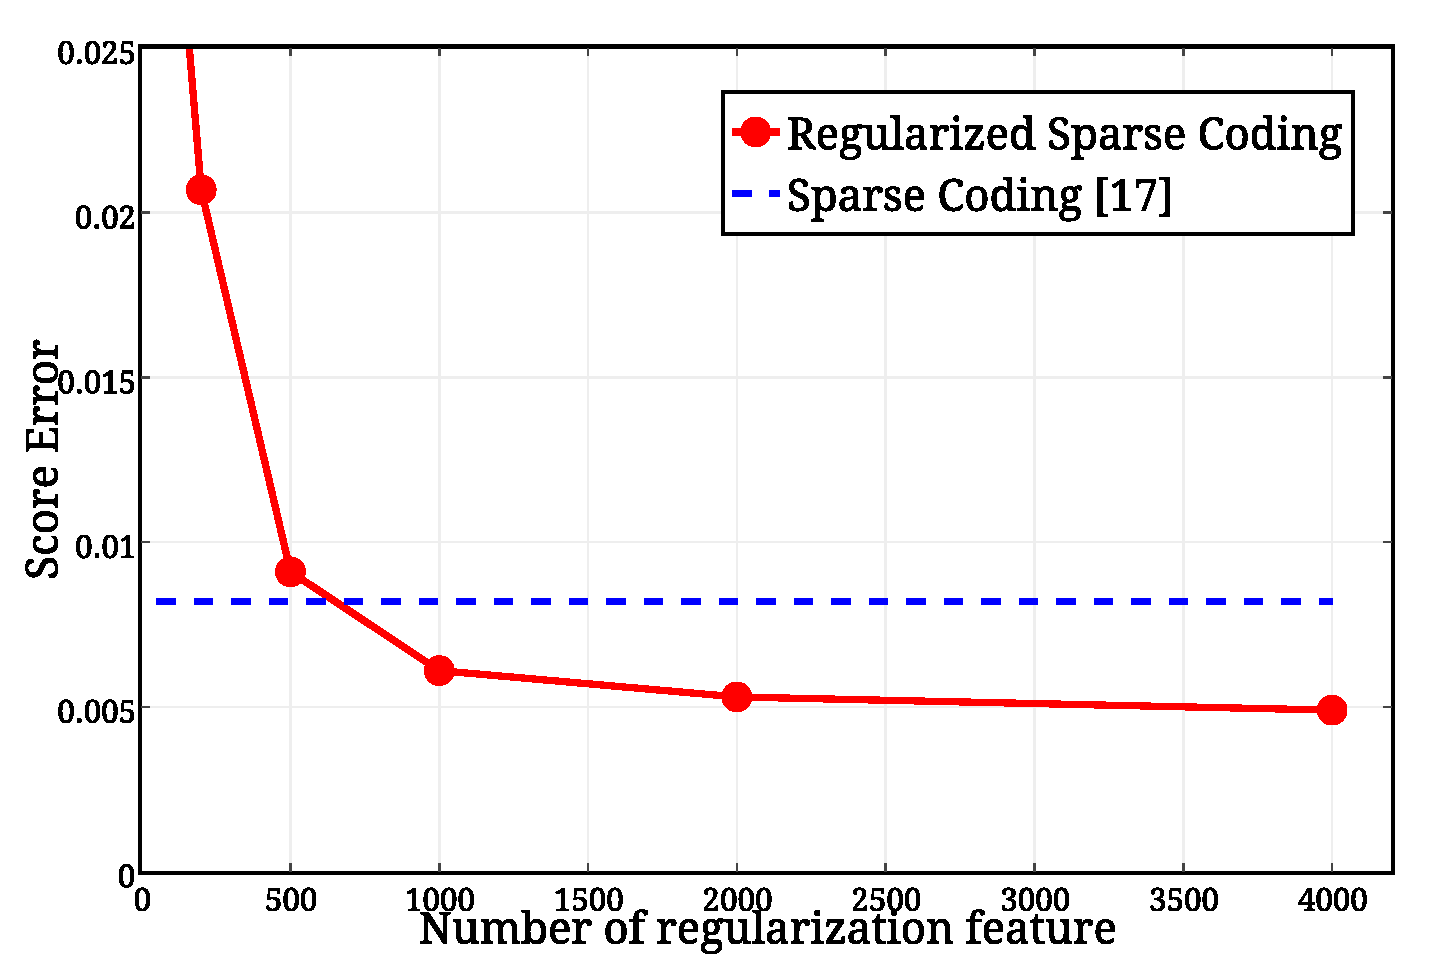
\includegraphics[width=0.48\textwidth]{featureUsage}
\caption{Effect of the number of regularization features used in Regularized Sparse Coding\protect\footnotemark[3]. As the solid line illustrates, the score error drops with more features involved. The dotted line is the original sparse coding method. Although sparse coding also has low score error, small difference of score error between the two method will result in a huge performance difference (mAP) in later experiments.}
\label{figFeatureUsage}
\end{figure}

\section{Performance Analysis}

\section{Scalability}

To compare sparse coding with our method, we conduct experiments on ILSVRC2013 ...


\chapter{Conclusion}
\label{c:conc}

In this work we proposed a method called Regularized Sparse Coding to speedup large scale object detection. Our method learns a codebook for the filters from part-based models and conduct operations only on the codebook to reduce computation. The original sparse coding method has accuracy loss problem when the number of classes grows larger, especially when a large speedup is required. Our work first introduces regularization process, which transforms filters and codebook into performance augmented space. Reconstruction in performance augmented space can minimize score map error of filters and achieve large speedup with negligible accuracy loss. To evaluate our method, we conduct experiments and compare our method with the sparse coding method \cite{song2012sparselet}. On VOC2012 we prove that our method can perform better than sparse coding especially when a large speedup is required. On ILSVRC2013 our method reaches a 16 times speedup using only 1.25\% memory with only 0.04 mAP loss compared to the original Deformable Part Model and outperforms the sparse coding method as well. To evaluate the effect of the number of filters on the speedup, we conduct experiments with different filter size and prove that deploying our method on larger filter size can have better accuracy-speedup trade off. Our method can also complement other methods which focus on reducing computation in the proposal extraction stage and parallel computation on GPUs to achieve more speedup. In future, we plan to apply our method on other applications, such as classification and segmentation, to provide speedup without accuracy loss and huge memory usage.


\appendix

\backmatter

\addcontentsline{toc}{chapter}{\bibname}
\bibliographystyle{abbrv}

% Your bibliography goes here
\bibliography{thesis}

\end{document}
